\documentclass[11pt]{cernrep}
\usepackage{graphicx,epsfig, url,cite,slashed}
\usepackage[utf8]{inputenc}
\usepackage[bookmarks,linktocpage]{hyperref}
\bibliographystyle{lesHouches}



\hypersetup{
   colorlinks=true,       % false: boxed links; true: colored links
   linkcolor=blue,        % color of internal links
   citecolor=red,         % color of links to bibliography
   filecolor=magenta,     % color of file links
   }

\begin{document}

\setlength\parindent{0pt}

\title{Recasting activities at LH2017}

\author{
Andy~Buckley$^{AB}$, 
Nishita~Desai$^{ND}$,
Benjamin~Fuks$^{BF1,BF2}$,
Philippe~Gras$^{PG}$, 
David~Grellscheid$^{DG}$,
Sabine~Kraml$^{SK}$,
Fabio~Maltoni$^{FM}$,
Olivier~Mattelaer$^{FM}$,
Luca~Perrozzi$^{LP}$,
Peter~Richardson$^{PR}$,
Sezen~Sekmen$^{SS}$
}
% Gabriel~Facini, 
% Jonathan~Butterworth, 
% Eric~Conte, 
% Pasquale~Musella, 
% Alexandra~Oliveira~Carvalho, 
% Ursula~Laa, 
% Kristin~Lohwasser,
% ???~Thrynova, 
% Efe~Yazgan, 
% Sylvain~Fichet
%}

\institute{
$^{LP}$ IPA at ETH Zurich, Switzerland\\
$^{AB}$ School of Physics \& Astronomy, University of Glasgow, UK\\
$^{BF1}$ Sorbonne Université, CNRS, Laboratoire de Physique Théorique et Hautes \'Energies, LPTHE, F-75005 Paris, France\\
$^{BF2}$ Institut Universitaire de France, 103 boulevard Saint-Michel, 75005 Paris, France \\
$^{PG}$ IRFU, CEA, Universit\'e Paris-Saclay, Gif-sur-Yvette\\
$^{FM}$ CP3/IRMP, Universit\'e Catholique de Louvain, chemin du cyclotron,2 1348 Louvain, Belgique\\
}
% $^2$ \dots\\

\maketitle

\begin{abstract}
The scope of this report is to document the advancements obtained on the recasting
activities and provide a first benchmark to compare different tools in reproducing ATLAS and CMS analysis results.
\end{abstract}

\section{Introduction}

Searches for new physics constitute a basic ingredient of the LHC physics program.
Their large number and variety pose severe challenges to both the experimental and theory communities.
In fact, hundreds of searches are performed by different collaborations, several final states are used,
while new ideas 
% on how 
to probe new models and non-trivial signatures and improve the sensitivity of existing searches constantly emerge.
The ultimate goal of this effort is to discover new physics if such
exists within the reach of the LHC, and to test the widest possible range of hypothetical new physics models.

A typical analysis defines quantities to classify events as signal
or background. They include properties of analysis objects such as
jets, electrons, muons, or global event variables such as object multiplicities,
transverse momenta or transverse masses.
An analysis can be very complex and feature many intricate definitions of object and event
variables, some of which cannot be expressed in closed algebraic form and must be defined
algorithmically. This complexity renders the task of visualizing, understanding, developing and
interpreting analyses increasingly challenging.

One obvious way to cope with this complexity is to devise ways to enforce absolute clarity in the description of analyses.
A discussion was started in the Les Houches PhysTeV workshop in 2011, and continued
thereafter within a wider group of LHC physicists, in order to determine what information is
crucial for describing an analysis. The outcome of this discussion was reported in the
''Recommendations for Presentation of LHC Results''~\cite{Brooijmans:2012yi,Kraml:2012sg,Brooijmans:2016vro}, and has been embraced by many LHC physicists.

The current practice in our community is to write an analysis in non-public computer codes,
which often rely on event objects specific to the experimental collaboration in question,
and then make public a description of the analysis via journal publications or other documents.

These efforts, which merit our great appreciation,
have significantly increased the scientific value of many important experimental results.

There is significant precedent for the effectiveness of such community standards. Several
accords have been established to standardize the communication of physics modeling information,
notably the Les Houches Event Accord (LHE)~\cite{Boos:2001cv,Alwall:2006yp} and the SUSY Les Houches Accord (SLHA)~\cite{Allanach:2008qq,Skands:2003cj}.
These, respectively, standardize the description of hard-process
particles in simulated collision events, and the details of all the parameters that define a new physics model point.
Both accords are widely used in high-energy physics and have greatly helped to
simplify and make more efficient the communication between physicists.
In recent years, the need for a standardized format was also underscored,
{\it i.e.} an “analysis description
accord”, capable of describing the contents of an analysis in an unambiguous way, which can
be fully exploited by the whole particle physics community.  The accord must be capable of
describing all object and event selections, as well as quantities such as efficiencies, analytic and
algorithmic observables, and advanced multivariate selections.
In the Les Houches PhysTeV workshop in 2015, a dedicated discussion has been initiated
on how such an accord can be realized~\cite{Brooijmans:2016vro}.
The important motivations and use-cases for a standard analysis description accord were envisaged as:
analysis preservation, analysis design, analysis review and communication, interpretation studies and analysis reimplementation, as well as easier comparison of analyses.
In addition, there are several desirable features which would further improve the utility
of the accord, which, however, may be nontrivial to simultaneously fulfill.  
The features required for the success of such an accord would be divided into basic requirements (public availability, completeness, longevity, correctness and validatability) and desirable features (human readability and writeability, self-contained, language independence, framework independence, support for combination of analyses).
Other proposals in this direction have been realized~\cite{Collaboration:2242860,recasting_atlas}.

Several discussions and progresses have been made, but the proposal is not yet final and has not been widely adopted yet.

% In the following sections we shall detail the use cases
% and design requirements of such an accord, and the general pros and cons of several approaches.

The scope of this report is to document the advancements obtained on the recasting
activities and provide a first benchmark to compare different tools in reproducing ATLAS and CMS analysis results
% The scope of this report, is to document the advancements obtained so far
% on the recasting activities, and the attempt for a first benchmark to compare different tools
% to reproduce several ATLAS and CMS analysis results 
provided through HEPDATA~\cite{Maguire:2017ypu}.
To test the reliability of this recasting approach, we realize feasibility studies of the implementation and portability of complicated multivariate techniques
(boosted decision trees, neutral networks, {\it etc.}) into the recasting frameworks featuring different approaches 
like detector smearing (Delphes~\cite{deFavereau:2013fsa}) results and simple object smearing.

Further improvements in the presentation of the results and their recastability
will include correlations among the signal systematics, 
as well as the possibility to provide unfolded distributions for key observables.
Finally, in the future it might become possible to directly use particle-level measurements to constrain new models.

% \section{Formats}
% Object efficiency tables : which format (HEPDATA?)

\section{Benchmarking tools and comparison strategy}

The idea behind the exercise described in this section is the implementation of
LHC analyses of increasing complexity, both in the language-independent format
(Analysis Description Format, LHADA Proposal) and frameworks like
CheckMate~\cite{Drees:2013wra,Cacciari:2005hq},
MadAnalysis~\cite{Conte:2012fm,Conte:2014zja,Dumont:2014tja}
and Rivet~\cite{Waugh:2006ip,Buckley:2010ar}, followed by a comparison of the results.
We choose analyses of ATLAS and CMS which have a detailed cutflow and detector effects provided in some form.
% , and possibly is already been implemented in the recasting codes CheckMate/MadAnalysis/Rivet/ATOM.
In the future it might be beneficial to use dedicated parsers to convert the analysis into different recasting codes.
Once the analysis are available in the needed format, we attempt to reproduce the new physics
interpretations presented in the original experimental research papers,
validating in this way our reimplementations.
A further step consists in the recasting of the analyses within diFFerent new
physics contexts and compare the results among the different frameworks.
A sketch of the recasting exercise workflow is presented in Fig.~\ref{fig:exercise}.

Aside the current scope of the exercise, it is interesting to check how the performance of the Delphes simulation behave across different phase spaces, since they are generally referred to as analysis-spedfic.


% \section{Analysis validation}
\begin{figure}
\begin{center}
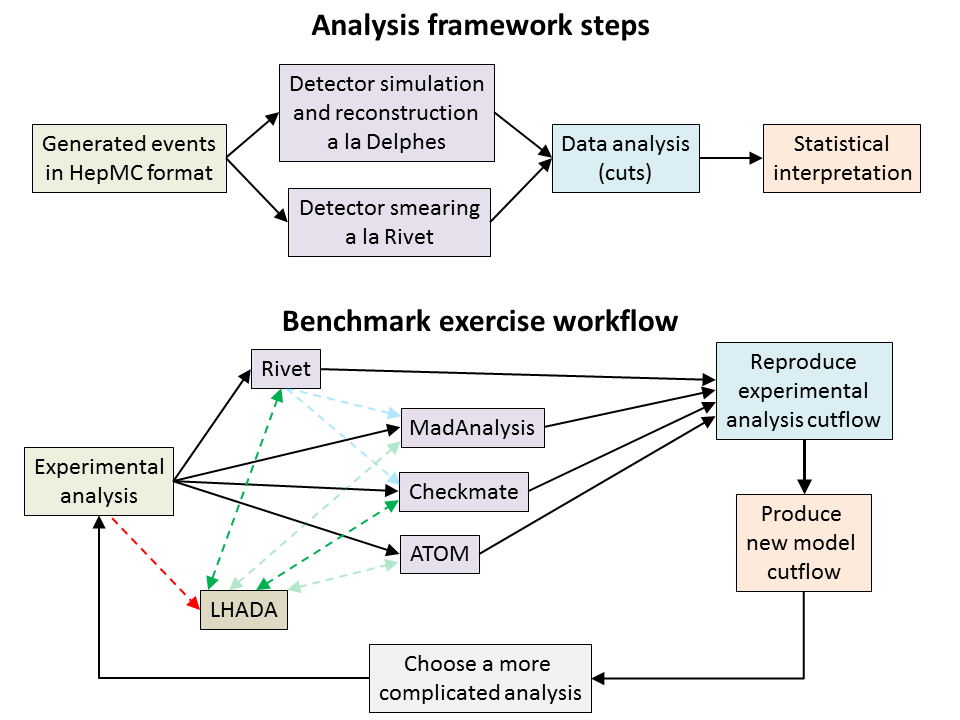
\includegraphics[width=0.65\textwidth]{figures/lhada_benchmarking_excersise.png}
 \caption{Sketch of the recasting exercise workflow.
}
\label{fig:exercise}
\end{center}
\end{figure}


\subsection{Analysis frameworks and tools}
In this section we describe the analysis frameworks and tools used for the comparison and benchmarking
% \subsection{ATOM}
% Atom is a general purpose framework for reinterpreting existing experimental analyses and designing new ones. Originally started as a fork of Rivet, Atom includes the possibility of describing detector effects by using transfer functions from truth-level objects to detector objects. In addition to providing a recasting framework, Atom emphasizes checking the validity of the extrapolations intrinsic in recasting a result from one BSM model to another. This is achieved via a flexible system warning the user of various conditions invalidating the results. On top of providing a database of existing BSM ATLAS and CMS analyses, LHC run I and II detector descriptions, while still being fully compatible with all Rivet analyses, Atom delivers tools for easily implementing new analyses, including an automatic validation system.

\subsubsection{CheckMate}
CheckMATE~\cite{Drees:2013wra,Cacciari:2005hq} takes simulated event files in .hep or .hepmc for any model as input and simply returns if the underlying model is `excluded' or `allowed' after
performing a detector simulation and testing various implemented analyses. The embedded AnalysisManager allows for the embedding of additional current and
prospective future LHC results from ATLAS and CMS which have not yet been implemented.
Detector effects are modeled by Delphes with a tune containing efficiency functions for lepton reconstruction and flavour tagging. The soon-to-be published version 2.0 of the code adds the possibility of using Pythia 8~\cite{Sjostrand:2007gs} to
generate supersymmetric events on-the-fly or to shower provided Les Houches
event files for any model. Currently, the collaboration is working on an extension to enable the on-the-fly simulation of events for any model.


\subsubsection{MadAnalysis}
MadAnalysis 5~\cite{Conte:2012fm,Conte:2014zja} is a generic user-friendly
framework for phenomenological investigations at particle colliders, {\it i.e.}
to perform physics analyses of Monte Carlo event files. While prospective
analyses of hard scattering events, parton showered events, hadronized events or
reconstructed events can be designed easily thanks to its Python-based
meta-language, MadAnalysis also allows for the recasting of LHC analyses on new
physics signals provided under the form of .hep and .hepmc event files. The
output here consists in the confidence level at which the model signals are
excluded.
Its Public Analysis Database~\cite{Dumont:2014tja} comprises a growing
collection of LHC analyses which have been implemented in the MadAnalysis 5
framework for the purpose of recasting. Delphes is used for the detector
simulation. For each implemented analysis, a detailed validation note is
provided and the public analysis database follows an open-source policy. Only
contributed codes provided with a detailed validation note are published, and
they are moreover citable via Inspire. The framework being integrated within
MadGraph5\_aMC@NLO~\cite{Alwall:2014hca}, it provides a full recast chain linking a model
and its associated signatures to limit setting.

\subsubsection{Rivet}
Originally developed as a toolkit for the validation of Monte Carlo event
generators, Rivet~\cite{Waugh:2006ip,Buckley:2010ar} (Robust Independent Validation of Experiment and
Theory) has become a standard for documenting (unfolded) Standard Model (SM)
measurements. The top and Higgs physics working groups of all LHC experiments
are increasingly providing Rivet routines for their analyses. Rivet analyses are
written in a user-friendly subset of C++11, and are picked up at runtime as
`plugin libraries'; they can be executed on an event stream either through a Python script interface, or by direct code interfacing to a C++ API.
The original SM-focused requirement of unfolded observables made Rivet
inappropriate for beyond the Standard Model (BSM) searches (other than those
using just jets and missing energy) until the addition of
detector-smearing/efficiency machinery in Rivet~2.5.0. This detector machinery provides equivalent efficiency effects to a Delphes-type simulation, and imitates the less important kinematic smearing of physics objects to within a few percent. A novel feature is that the Rivet detector implementation allows for using
different jet algorithms, lepton and b-tagging operating points, full-detailed object isolation algorithms, and resolutions/efficiencies specific to each
analysis procedure and event selection. This hence allows for a more accurate detector modelling and more robust analysis preservation than `global' detector simulations in addressing some experiment requests for `official fast-sim' tools. The aim is to encourage Rivet code provision directly from BSM data analysers, as is already the case for SM results: additional tools to assist BSM analysis implementation are being added on request.

\subsubsection{Generic Analysis Description Proposal}
A description of the Generic Analysis Description Proposal and its recent developments in contained in section~\ref{LHADA} of the proceedings.

\section{Analyses benchmarking, comparisons and results}

\subsection{An ATLAS search for supersymmetry in a final
state with jets and missing energy (13 TeV, 3.2~fb$^{-1}$)}

\begin{table*}
\footnotesize
 \centering
  \begin{tabular}{ | l || l | l | l || l | l | l || l | }
\hline
    &  \multicolumn{3}{c||}{\bf Rivet} & \multicolumn{3}{c||}{\bf MadAnalysis 5} &   {\bf CheckMATE}   \\ \hline
  Description       & \#evt & tot.eff & rel.eff & \#evt & tot.eff & rel.eff &   tot.eff   \\ \hline \hline
{\bf 2jl cut-flow}                  & 31250 & 1 & - & 31250 & 1 & - & \   \\ \hline
Pre-sel+MET+pT1   & 28592 & 0.91 & 0.91 & 28626 & 0.92 & 0.92 & \   \\ \hline
Njet              & 28592 & 0.91 & 1 & 28625 & 0.92 & 1 & \   \\ \hline
Dphi\_min(j,MET)   & 17297 & 0.55 & 0.6 & 17301 & 0.55 & 0.6 & \   \\ \hline
pT2               & 17067 & 0.55 & 0.99 & 17042 & 0.55 & 0.99 & \   \\ \hline
MET/sqrtHT        & 8900 & 0.28 & 0.52 & 8898 & 0.28 & 0.52 & \   \\ \hline
m\_eff(incl)       & 8896 & 0.28 & 1 & 8897 & 0.28 & 1 & \   \\ \hline
\hline
{\bf 2jm cut-flow} & 31250 & 1 & - & 32150 & 1 & - & 1  \\ \hline
Pre-sel+MET+pT1   & 28472 & 0.91 & 0.91 & 28478 & 0.91 & 0.91 & 0.91  \\ \hline
Njet              & 28472 & 0.91 & 1 & 28477 & 0.91 & 1 & 0.91  \\ \hline
Dphi\_min(j,MET)   & 22950 & 0.73 & 0.81 & 22889 & 0.73 & 0.8 & 0.73  \\ \hline
pT2               & 22950 & 0.73 & 1 & 22889 & 0.73 & 1 & 0.73  \\ \hline
MET/sqrtHT        & 10730 & 0.34 & 0.47 & 10710 & 0.34 & 0.47 & 0.33  \\ \hline
m\_eff(incl)       & 10630 & 0.34 & 0.99 & 10609 & 0.34 & 0.99 & 0.32  \\ \hline
\hline
{\bf 2jt cut-flow} & 31250 & 1 & - & 31250 & 1 & - & \   \\ \hline
Pre-sel+MET+pT1   & 28592 & 0.91 & 0.91 & 28626 & 0.92 & 0.92 & \   \\ \hline
Njet              & 28592 & 0.91 & 1 & 28625 & 0.92 & 1 & \   \\ \hline
Dphi\_min(j,MET)   & 17297 & 0.55 & 0.6 & 17301 & 0.55 & 0.6 & \   \\ \hline
pT2               & 17067 & 0.55 & 0.99 & 17042 & 0.55 & 0.99 & \   \\ \hline
MET/sqrtHT        & 5083 & 0.16 & 0.3 & 5098 & 0.16 & 0.3 & \   \\ \hline
Pass m\_eff(incl)  & 4861 & 0.16 & 0.96 & 4889 & 0.16 & 0.96 & \   \\ \hline
		\end{tabular}
 \caption{Number of events surviving each selection, total and relative
  selection efficiencies as obtained with Rivet and MadAnalysis 5 for the dijet
  signal regions of the multijet+missing energy ATLAS analysis of
  Ref.~\cite{Aaboud:2016zdn}. Partly available Checkmate results for the total
  efficiencies are also indicated.}
	\label{tab:1605.03814-2j}
\end{table*}

In the analysis of Ref.~\cite{Aaboud:2016zdn}, the ATLAS collaboration targets
the production of the strongly-interacting superpartners of the Standard Model
QCD partons, followed by their decay into jets and missing energy carried by
neutralinos. 3.2~fb$^{-1}$ of proton-proton LHC collisions at a center-of-mass
energy of 13~TeV are analyzed.

\begin{table*}
\begin{tabular}{ | l || l | l | l || l | l | l || l | }
\hline
    &  \multicolumn{3}{c||}{\bf Rivet} & \multicolumn{3}{c||}{\bf MadAnalysis 5} &   {\bf CheckMATE}   \\ \hline
  Description       & \#evt & tot.eff & rel.eff & \#evt & tot.eff & rel.eff &   tot.eff   \\ \hline \hline
\hline
{\bf 4jt cut-flow} & 31250 & 1 & - & 31250 & 1 & - & 1  \\ \hline
Pre-sel+MET+pT1   & 28592 & 0.91 & 0.91 & 28626 & 0.92 & 0.92 & 0.91  \\ \hline
Njet              & 27322 & 0.87 & 0.96 & 27128 & 0.87 & 0.95 & 0.87  \\ \hline
Dphi\_min(j,MET)   & 18929 & 0.61 & 0.69 & 18829 & 0.6 & 0.69 & 0.6  \\ \hline
pT2               & 18715 & 0.6 & 0.99 & 18825 & 0.6 & 1 &     --       \\ \hline
pT4               & 16610 & 0.53 & 0.89 & 16430 & 0.53 & 0.87 & 0.52  \\ \hline
Aplanarity        & 11849 & 0.38 & 0.71 & 11395 & 0.36 & 0.69 & 0.36  \\ \hline
MET/m\_eff(Nj)     & 8334 & 0.27 & 0.7 & 7971 & 0.26 & 0.7 & 0.25  \\ \hline
m\_eff(incl)       & 7201 & 0.23 & 0.86 & 6972 & 0.22 & 0.87 & 0.21  \\ \hline
\hline
{\bf 5j cut-flow} & 31250 & 1 & - & 31250 & 1 & - & 1 \\ \hline
Pre-sel+MET+pT1   & 28592 & 0.91 & 0.91 & 28626 & 0.92 & 0.92 & 0.91 \\ \hline
Njet              & 21234 & 0.68 & 0.74 & 21185 & 0.68 & 0.74 & 0.68 \\ \hline
Dphi\_min(j,MET)   & 14294 & 0.46 & 0.67 & 14292 & 0.46 & 0.67 & 0.45 \\ \hline
pT2               & 14146 & 0.45 & 0.99 & 14289 & 0.46 & 1 &    --       \\ \hline
pT4               & 13229 & 0.42 & 0.94 & 13228 & 0.42 & 0.93 & 0.42 \\ \hline
Aplanarity        & 9836 & 0.31 & 0.74 & 9576 & 0.31 & 0.72 & 0.3 \\ \hline
MET/m\_eff(Nj)     & 4643 & 0.15 & 0.47 & 4506 & 0.14 & 0.47 & 0.13 \\ \hline
m\_eff(incl)       & 4620 & 0.15 & 1 & 4476 & 0.14 & 0.99 & 0.13 \\ \hline
\hline
{\bf 6jm cut-flow} & 31250 & 1 & - & 31250 & 1 & - & 1  \\ \hline
Pre-sel+MET+pT1   & 28592 & 0.91 & 0.91 & 28626 & 0.92 & 0.92 & 0.91  \\ \hline
Njet              & 13235 & 0.42 & 0.46 & 13236 & 0.42 & 0.46 & 0.41  \\ \hline
Dphi\_min(j,MET)   & 8520 & 0.27 & 0.64 & 8553 & 0.27 & 0.65 & 0.26  \\ \hline
pT2               & 8436 & 0.27 & 0.99 & 8551 & 0.27 & 1 &    --        \\ \hline
pT4               & 8135 & 0.26 & 0.96 & 8217 & 0.26 & 0.96 & 0.25  \\ \hline
Aplanarity        & 6365 & 0.2 & 0.78 & 6307 & 0.2 & 0.77 & 0.19  \\ \hline
MET/m\_eff(Nj)     & 2675 & 0.09 & 0.42 & 2665 & 0.09 & 0.42 & 0.08  \\ \hline
m\_eff(incl)       & 2670 & 0.09 & 1 & 2656 & 0.08 & 1 & 0.08  \\ \hline
\hline
{\bf 6jt cut-flow} & 31250 & 1 & - & 31250 & 1 & - & \   \\ \hline
Pre-sel+MET+pT1   & 28592 & 0.91 & 0.91 & 28626 & 0.92 & 0.92 & \   \\ \hline
Njet              & 13235 & 0.42 & 0.46 & 13236 & 0.42 & 0.46 & \   \\ \hline
Dphi\_min(j,MET)   & 8520 & 0.27 & 0.64 & 8553 & 0.27 & 0.65 & \   \\ \hline
pT2               & 8436 & 0.27 & 0.99 & 8551 & 0.27 & 1 & \   \\ \hline
pT4               & 8135 & 0.26 & 0.96 & 8217 & 0.26 & 0.96 & \   \\ \hline
Aplanarity        & 6365 & 0.2 & 0.78 & 6307 & 0.2 & 0.77 & \   \\ \hline
MET/m\_eff(Nj)     & 3900 & 0.12 & 0.61 & 3839 & 0.12 & 0.61 & \   \\ \hline
m\_eff(incl)       & 3715 & 0.12 & 0.95 & 3672 & 0.12 & 0.96 & \   \\ \hline
 \end{tabular}
 \caption{Same as in Table~\ref{tab:1605.03814-2j} but for the signal regions
  targeting final states containing four, five and six jets.}
	\label{tab:1605.03814-nj}
\end{table*}

The analysis focuses on jets reconstructed by means of the anti-$k_T$
algorithm~\cite{Cacciari:2008gp} with a radius parameter set to $R=0.4$, with
a transverse momentum larger than 20~GeV and a pseudorapidity $|\eta|<2.8$.
Events featuring loosely reconstructed electrons and muons are vetoed.
Event preselection requires a significant amount of missing energy,
$\slashed{E}_T > 200$~GeV and the transverse-momentum of the leading jet is
imposed to be larger than 200~GeV and 300~GeV if two or more than two jets are
reconstructed, respectively.

The analysis is then divided into seven signal regions focusing on different jet
multiplicities (from 2 to 6) with different transverse-momentum thresholds. The
missing transverse momentum is then enforced to be well separated from the
leading reconstructed jets, and its significance is constrained for events
featuring only two jets. For cases where at least four jets are reconstructed,
additional selections on the aplanarity variable
% ~\cite{Chen:2011ah} 
and the effective mass, {\it i.e} the scalar sum of the transverse momenta of the
reconstructed and the missing transverse energy.

% More information of the MadAnalysis 5 implementation of this analysis can be
% found in Refs.~\cite{Banerjee:2017wxi,ma5-1605.03814}. 
The comparison of
predictions for the cutflows as obtained with MadAnalysis 5 and Rivet are
reported in Table~\ref{tab:1605.03814-2j} and Table~\ref{tab:1605.03814-nj} for
all seven signal regions. The pseudo-data sample have been generated by using MadGraph5\_aMC@NLO and Pythia8 \cite{Sjostrand:2014zea}. The tables include the total number of events
surviving each selection, the associated cut efficiency and the total efficiency
evaluated with respect to the initial number of events. Partially available
Checkmate results are also indicated for what concern the total efficiencies and
for a few signal regions.

An excellent agreement between the three codes has been obtained.

\subsection{An ATLAS search for dark matter in the monophoton final state
  (13~TeV,  36.1~fb$^{-1}$)}

In the analysis of Ref.~\cite{Aaboud:2017dor}, the ATLAS collaboration has
searched for dark matter when it is produced in association with a very
energetic photon. The search results have been reinterpreted in dark matter
simplified scenarios in which a pair of dark matter particles is produced in
association with a photon arising from initial state radiation. 36.1~fb$^{-1}$
of proton-proton LHC collisions at a center-of-mass energy have been analyzed.

The analysis requires the presence of at least one tightly-isolated photon with
a transverse energy $E_T > 150$~GeV and with a pseudorapidity satisfying
$|\eta| < 2.37$, the pseudorapidity region $1.37 < |\eta| < 2.37$ being
excluded. Events featuring loose eletrons and muons and more than one jets with
a transverse momentum larger than 30~GeV and a pseudorapidity $|\eta|<4.5$ are
vetoed. As in the previous analysis, jets are reconstructed by means of the
anti-$k_T$ algorithm~\cite{Cacciari:2008gp}  and a radius parameter set to
$R=0.4$. In addition, event selection requires a missing transverse energy
significance larger than 8.5~GeV$^{1/2}$, and the missing transverse momentum
has top be well separated from the photon and the jet (for events featuring one
reconstructed jet).

Five signal regions are defined according to different requirements on the
amount of missing transverse energy, namely three inclusive regions and two
non-overlapping exclusive regions.

% More information on the MadAnalysis 5 implementation of this analysis can be
% found in Ref.~\cite{inspire_monophoton}. 
In Table~\ref{tab:1704.03848}, we
compare the total number of events surviving each selection, the associated cut
efficiency and the total efficiency evaluated with respect to the initial number
of events as obtained with MadAnalysis 5 and Rivet. Whilst a fair agreement is
obtained between two codes, differences of 5\%-10\% are observed for a cuople of
cuts. This can be traced back to the missing energy modeling that is complicated
to reproduce.

\begin{table*}
 \centering
  \begin{tabular}{ | l || l | l | l || l | l | l | }
\hline
                  &  \multicolumn{3}{c||}{\bf Rivet} & \multicolumn{3}{c||}{\bf MadAnalysis 5}    \\ \hline

Description       & \#evt & tot.eff & rel.eff & \#evt & tot.eff & rel.eff    \\ \hline \hline

Initial                    &  	1198	& 1		  & -     & 1198	& 1	 &    -      \\ \hline
ETmiss $>$ 150 GeV           &   	798.3	& 0.67	& 0.67	& 736	& 0.61 &  0.61     \\ \hline
Photon w/ ET $>$ 150 GeV     &   	703.5	& 0.59	& 0.88	& 700	& 0.58 &  0.95     \\ \hline
Pass Tight photon          &   	598.1	& 0.50	& 0.85	& 658	& 0.55 & 	0.94     \\ \hline
Pass Isolated photon       &   	598.1	& 0.50	& 1.00	& 620	& 0.52 & 	0.94     \\ \hline
Pass $\delta\phi$(gamma,MET) $>$ 0.4 &   	597.5	& 0.50	& 1.00	& 596	& 0.50 & 	0.96     \\ \hline
Pass MET/sqrt(SET) $>$ 8.5   &   	538.2	& 0.45	& 0.90	& -	  &  -   &     	     \\ \hline
Pass Jet veto              &   	476.8	& 0.40	& 0.89	& 461	& 0.38 & 	0.77     \\ \hline
Pass Lepton veto           &   	475.5	& 0.40	& 1.00	& 460	& 0.38 & 	1.00     \\ \hline
  \end{tabular}
 \caption{Number of events surviving each selection, total and relative
  selection efficiencies as obtained with Rivet and MadAnalysis 5 for the SRI1
  signal region of the monophoton ATLAS analysis of Ref.~\cite{Aaboud:2017dor}.}
 \label{tab:1704.03848}
\end{table*}


\subsection{A CMS search for electroweakinos in multileptonic final states
  (13~TeV, 35.9~fb$^{-1}$)}

In the analysis of Ref.~\cite{Sirunyan:2017lae}, the CMS collaboration
investigates potential hints for electroweakinos, when the latter decays into
leptons and missing energy carried away by neutralinos. The search analyzes
35.9~fb$^{-1}$ of LHC proton-proton collisions at a center-of-mass energy of
13~TeV.

The CMS search preselects events featuring at least two isolated leptons
(electrons or muons) with soft transverse-momentum rquirements or a single
lepton with harder $p_T$ requirements, which allows one to get sensitivity to
topologies featuring hadronic taus. The analysis selection feature final states
with eother two, three or four leptons and little hadronic activity.

The analysis is subdivided into numerous signals regions and a small number of
aggregated signal regions.

A first class of signal regions requires a same-sign
dilepton where each lepton have a transverse momentum larger than 25~GeV
(20~GeV) for the leading electron (muon) and than 15~GeV (10~GeV) for the
subleading electron (muon). The amount of missing energy is constrained to be
larger than 60~GeV, and events compatible with a $WZ$ event involving a looser
lepton and an opposite-sign dilepton compatible with a $Z$-boson or a low-mass
resonance are vetoed. Events are allowed to feature at most one jet with
a transverse momentum larger than 40~GeV and a pseudorapidity $|\eta|<2.4$,
where jets are reconstructed by means of the anti-$k_T$
algorithm~\cite{Cacciari:2008gp} with a radius parameter set to $R=0.4$.
Additional selections on the missing energy, the transverse mass evaluated from
the transverse momentum of each lepton and the missing momentum and the $p_T$ of
the dilepton system are imposed and allow for the definition of 30 independent
signal regions.

Events featuring three or more leptons are required to contain more than 50~GeV
of missing energy and at most two hadronic tau candidates. 123 signal regions
are defined, depending on the number of leptons, their respective flavors, the
their elcetric charge, amount of missing energy, the value of the $m_{T2}$
variable~\cite{Lester:1999tx} and the invariant mass of the possible lepton
pairs.

The same observables are then used to define 8 aggregated signal regions.

The analysis has been implemented 
% in MadAnalysis 5 but the lack of
% information from CMS renders 
% its validation complicated.
in the recasting codes and the validation is ongoing.

\subsection{A CMS search for top squarks in single leptonic events (13~TeV,
  35.9~fb$^{-1}$)}

In the analysis of Ref.~\cite{Sirunyan:2017xse}, the CMS collaboration studies
potential hints for the production of a pair of top squarks that each decays
into a top quark and missing energy carried away by a neutralino. This search
focuses on top-antitop system further decaying semi-leptonically, the lepton
being either a muon or an electron, and investigate 35.9~fb$^{-1}$ of LHC
proton-proton collisions at a center-of-mass of 13~TeV.

The analysis requires the presence of a single isolated lepton with a transverse
momentum larger than 20~GeV and a pseudorapidity satisfying $|\eta| < 1.442$ and
2.4 for electrons and muons respectively. Jets are reconstructed by means of the
anti-$k_T$ algorithm~\cite{Cacciari:2008gp} with a radius parameter set to
$R=0.4$, and only jets with a transverse momentum larger than 30~GeV and a
pseudorapidity $|\eta| < 2.4$ are considered. The event selection asls for the
presence of at least two jets, with at least one of the reconstructed
jets is required to be $b$-tagged. Further requirements are then imposed on the
transverse mass of the lepton-missing energy system and a veto is iplemented so
that events featuring a second loosely isolated leptons are rejected. Finally,
the missing energy is imposed to be well separated in azimuth from the two
leading jets.

The analysis defines to categories of signal regions. The first of these
categories characterize events relatively to the number of jets, the missing
transverse energy, the invariant mass of the lepton-leading $b$-jet system and
the topness variable~\cite{Graesser:2012qy}. The second class of signal regions are
design to select featuring a hard initial-state radiation jet that boosted the
supersymmetric system. The events are required to feature at least 5 jets, the
leading jet being a light jet, and the lepton cannot have a transverse momentum
greater than 150~GeV and be to far from the missing transverse momentum. The
two leading jets are finally imposed to be quite separated from the missing
momentum, and the events are categorized according to the amount of missing
energy.

Implementations of this analysis in the recasting codes is ongoing. 


\section*{CONCLUSIONS}
A first benchmark to compare different recasting tools in reproducing ATLAS and CMS analysis results has been provided.
In general, good agreement is found between the different frameworks and detector simulation techniques.
The completion of the studies together with recasting of other analyses will shed more light
on the reliability of the methods in cases where extreme phase spaces and more complicated analysis techniques.

% \section*{ACKNOWLEDGEMENTS}
% We acknowledge the acknowledgements.

\bibliography{sample_bib}

\end{document}
